\section{Software Architecture}
In this section, I briefly describe the software architecture of the complete \pkg{StochBB} framework as shown in Fig. \ref{fig:arch}. 

\begin{figure} [!ht]
 \centering
 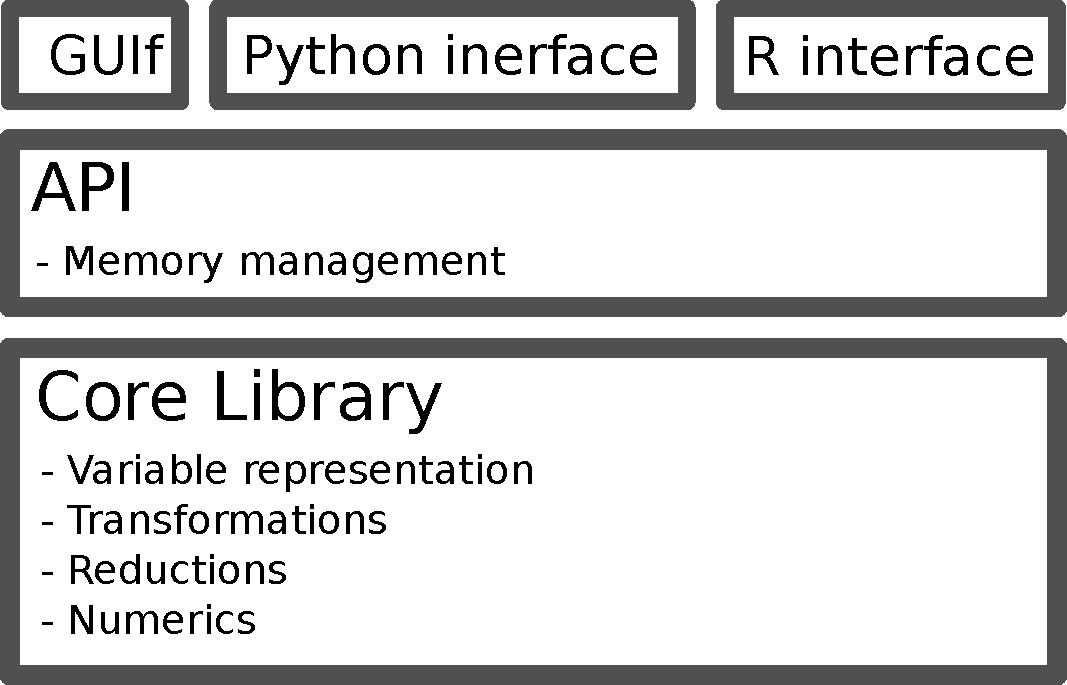
\includegraphics[width=0.5\textwidth]{fig/arch.pdf}
 \caption{Overview of the \pkg{StochBB} software architecture.} \label{fig:arch}
\end{figure}

The foundation of the complete framework is formed by the \pkg{StochBB} core library. This C++ library implements the core functionality of the system. Prominent elements are classes representing the atomic random-variable instances and parametric distributions as well as derived variables (e.g., sums of random variables) and their distributions (e.g., convolution densities).  Together, these classes form the representation of a complex system of dependent random variables. Analytic solutions for some marginal distributions are obtained by reduction and transformation operations performed on the system representation. Also these operations are part of the core library. Finally a set of numerical algorithms (e.g., numerical convolution and integrals) are implemented in the core library for obtaining numerical approximations of densities which cannot be derived analytically. 

Using the core library directly would be rather complicated as the C++ does not provide means of automatic memory management by itself. For easing the usage of the core library an application programming interface is provided above the core library that encapsulates all objects of the core library into container classes. These container classes then implement an automatic memory management by means of a \emph{mark-and-sweep} garbage collector \cite[e.g.,][]{Aho2007}. This API (described in the next section) is then used to provide interfaces to the Python and R programming language as well as implementing a graphical user interface (GUI) application also described below.